\colorlet{chaptergrey}{gray}
\chapter[Kinematically misaligned galaxies in IllustrisTNG]{Kinematic misalignment in TNG}
\label{ch:halo_assembly}
\vspace{-5.25in}
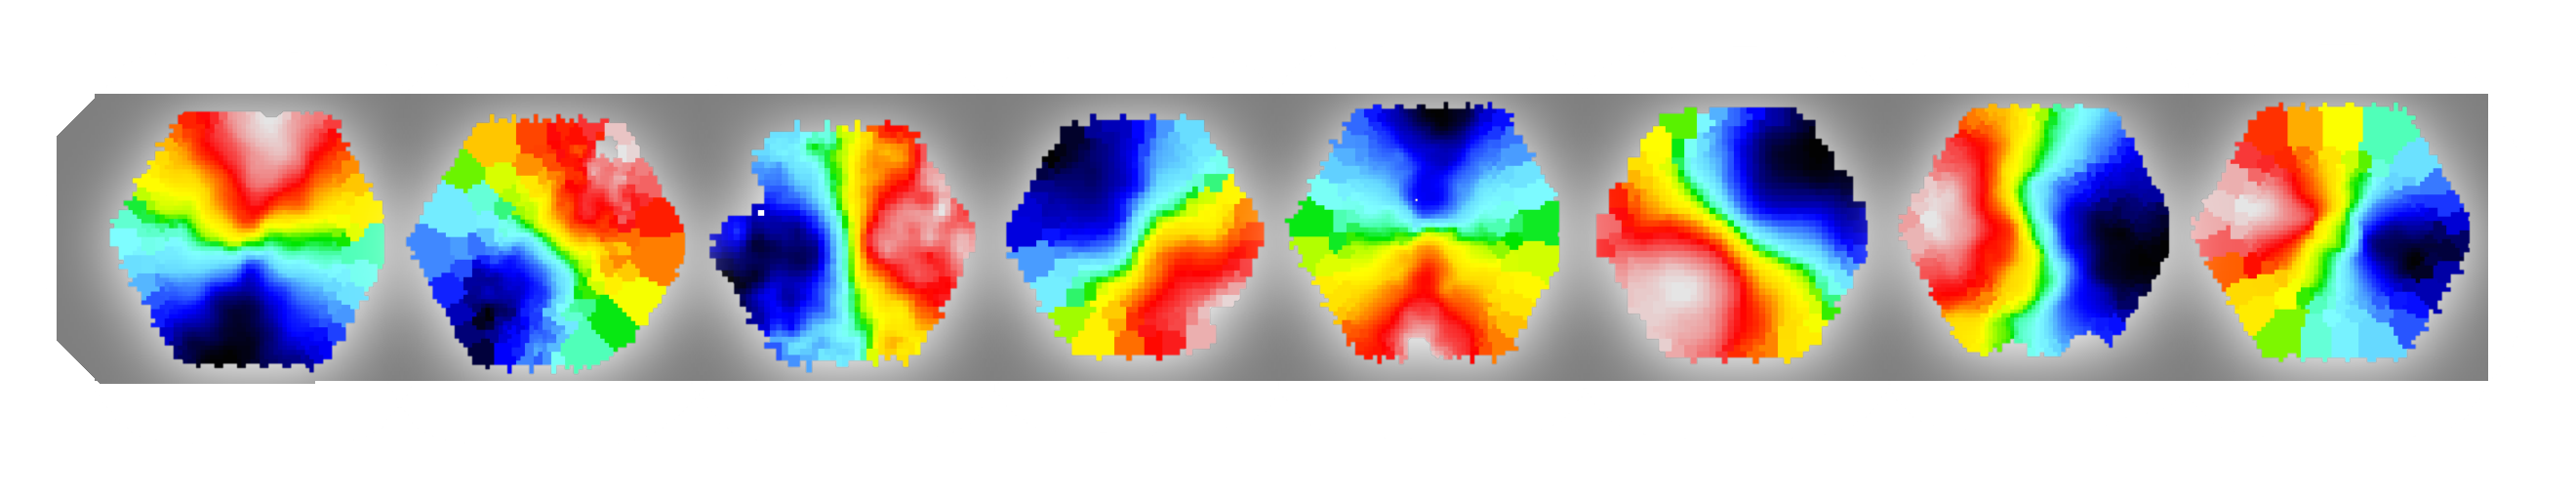
\includegraphics[height=1.39in]{thesis/latex/misalignment_MaNGA/kin_mis_chapter_heading_grey.pdf}
\vspace{3in}

\epigraph{This chapter is based on Duckworth, Tojeiro and Kraljic, in MNRAS, 492, Issue 2, 2020 and Duckworth, Starkenburg, Genel, Davis, Habouzit, Kraljic and Tojeiro (submitted). Here we investigate kinematically misaligned galaxies in the cosmological scale simulation IllustrisTNG. We make direct comparison to observations and investigate the relationship of misalignment identified at $z=0$ with the evolutionary histories of stellar angular momentum and halo spin.}

\section{Introduction}
\red{motivate the comparison of hydrodynamical simulations to observations with empathsis of angular momentum (genel, dephillipis, starkenburg, khim.}

In this chapter we describe the construction of a mock MaNGA sample created in the hydrodynamical simulation of IllustrisTNG. \S\ref{sec:sim_data_TNG} introduces the IllustrisTNG simulation and the creation of the mock observational sample. \S\ref{}

\section{Simulation data} \label{sec:sim_data_TNG}
\subsection{IllustrisTNG} 
The IllustrisTNG project \citep{marinacci18,naiman18,nelson18,pillepich18b,springel18} is a suite of magneto-hydrodynamic cosmological scale simulations incorporating an updated comprehensive model for galaxy formation physics \citep[as decribed in][]{weinberger17,pillepich18a} and making use of the moving-mesh code \texttt{AREPO} \citep{springel10,pakmor11,pakmor13}. For this work, we use the highest resolution fiducial run of TNG100 which follows the evolution of 2 x 1820$^3$ resolution elements within a periodic cube with box lengths of 110.7 Mpc (75 h$^{-1}$ Mpc). This corresponds to an average mass resolution of baryonic elements of 1.4 x 10$^6 \mathrm{M_{\odot}}$ and 7.5 x 10$^6 \mathrm{M_{\odot}}$ for dark matter. Here we make use of public data from the IllustrisTNG project \citep[as described in][]{nelson2019}.

Structure in TNG100 is identified into haloes and subhaloes as follows. Haloes (also referred to as FoF haloes or Groups) are found from a standard friends-of-friends (FoF) algorithm \citep{davis85} with linking length $b=0.2$. The FoF algorithm is run on the dark matter particles, and the other types (gas, stars, BHs) are attached to the same groups as their nearest DM particle. Each halo is then divided into gravitationally bound subhaloes through the subfind algorithm \citep{springel01}. In short, subfind defines `subhaloes' as locally over-dense and self-bound particle groups as distinct objects within given FoF haloes. We consider all subhaloes at $z=0$ containing a minimum stellar mass of $\mathrm{M_{\ast}} = 10^{8.5} \mathrm{M_{\odot}}$ to potentially make up our mock MaNGA like sample. Since we are typically considering the stellar component of these subhaloes for our mock observations, we will refer to these as TNG100 galaxies.

\subsection{Matching to MaNGA sample}
To construct a mock MaNGA sample we select representative subhaloes from TNG100. For every MaNGA galaxy, we find the TNG100 galaxy with the most similar stellar mass, size and SDSS $g - r$ colour. In this instance, stellar mass is defined by the total mass of stellar particles within a radius of 2 stellar effective radii. The SDSS $g - r$ colour is found using the prescription outlined in \citet{nelson18}. Here we describe the general process, while we direct the reader to \citet{nelson18} for more detail. Each stellar particle in the simulation is modelled as a single-burst simple stellar population. This is converted into a population spectrum using FSPS \citep{conroy2009,conroy2010,foreman_mackey2014} which is convolved with the pass-bands for SDSS colours. We use model C \citep[as described in][]{nelson18} which also includes models for unresolved and resolved dust. We use sizes following the prescription of \citet{genel2018}, which use a projected half light radius. The SDSS bands are constructed as above and are used to define circular half light radii for each SDSS band along X, Y and Z projections of the box. We use the $r-$band half light radius projected perpendicular to the XY plane, consistent with the line of sight of the mock MaNGA observation.

The matching is done through finding the closest neighbour in a normalised space with dimensions of the matched properties. If multiple MaNGA objects match to a given TNG100 galaxy then the absolute nearest neighbour is selected and the MaNGA object is assigned to its second nearest neighbour. The process is iterated until all have unique matches. 

The galaxy is then assigned the same bundle size IFU as the matched MaNGA galaxy with the corresponding angular resolution. The galaxy is then `observed' (see \S\ref{sec:mock_obs}) at a distance so that the angular footprint of the assigned IFU covers the same number of physical effective radii for the mock galaxy as the matched observation. 

\subsection{Mock observations} \label{sec:mock_obs}
We convert each galaxy in TNG100 into a mock MaNGA observation, as follows:

We take the raw particle/cell data of gas and stars and project on the XY plane (i.e. z-direction is the line of sight). Since there is no preferred direction in the simulation, this corresponds to a `random' viewing angle of each galaxy. We bin particles corresponding to the angular resolution of spaxels in MaNGA (0.5 arcsec/pixel), in the distinct hexagonal footprint of MaNGA observations. In each bin, we calculate the mean velocity, velocity dispersion and total flux for all particles. 

Since we include all particles along the line of sight, we must take care in interpreting the absolute values of flux, since none is lost due to obscuration. We, however, do not use the flux values calculated here in our work.

In order to estimate the typical noise associated with a MaNGA observation, we compute radial profiles of the signal to noise ratio (SNR) for all MaNGA observations of a given IFU size. MaNGA has 5 different IFU sizes corresponding to bundles of 19, 37, 61, 91 and 127 fibres. MaNGA provides estimates of the SNR for every spaxel in each observation in the $g$-band. Figure \ref{fig:noise_profile} shows the azimuthally averaged SNR profiles for all MaNGA observations of each fibre bundle size. We fit a logarithmic function to each profile, which is used to assign noise to the mock observations. Noise is drawn for each pixel from a normal distribution using the median and standard deviation of the fitted logarithmic radial profile.

\begin{figure}
    \centering
	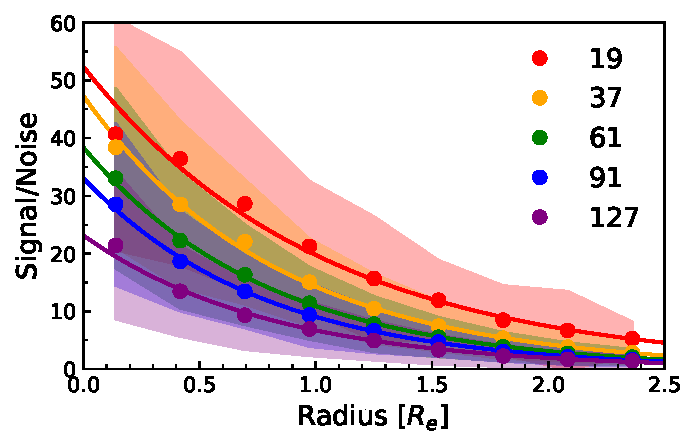
\includegraphics[width=0.95\linewidth]{misalignment_TNG/noise_profiles_ifusize.pdf}
    \caption{Average signal to noise profiles for each IFU size for all MaNGA MPL-8 observations. The circles show the median value for each radius bin with the shaded region corresponding to the standard deviation. The solid line corresponds to an logarithmic parametric fit to the data points, used in sampling the noise profile for the mock observations.}
    \label{fig:noise_profile}
\end{figure}

In order to simulate the effects of the point spread function (PSF), we then convolve our binned particle data with a Gaussian kernel. MaNGA observations typically have a $g$-band PSF which can be fit with a Gaussian of $\sim 2-3''$ full width half maximum (FWHM). We take all our mock observations to have a PSF modelled by a Gaussian with a 2$''$ FWHM. The spatial scale of the simulation is effectively set by the gravitational softening length of both the DM and stellar particles at 0.5h$^{-1}$ kpc = 0.74 kpc. This is approximately a factor of two (four) lower than the spatial sampling (PSF) of a typical MaNGA observation. The typical spatial resolution of star forming gas cells in TNG100 is of order $\sim$200pc and therefore suitable for our mock observations. We direct the reader to Figure 1 in \citet{pillepich2019} for further details (scale by a factor of $16^{1/3}$ for TNG100). \red{Do you direct readers elsewhere for a thesis?}

We fit position angles to MaNGA observations that have been Voronoi binned so that bins contain a minimum S/N $\sim 10$. To maintain consistency and avoid spurious individual particles biasing measurements, we also Voronoi bin our mock observations so that a minimum of 5 particles is contained within a given bin, again using the routine of \citet{cappellari2003}. Figure \ref{fig:example_obs} shows example stellar (and gas) velocity and dispersion fields along with normalised $r$-band flux, after our processing.

\begin{figure*}
	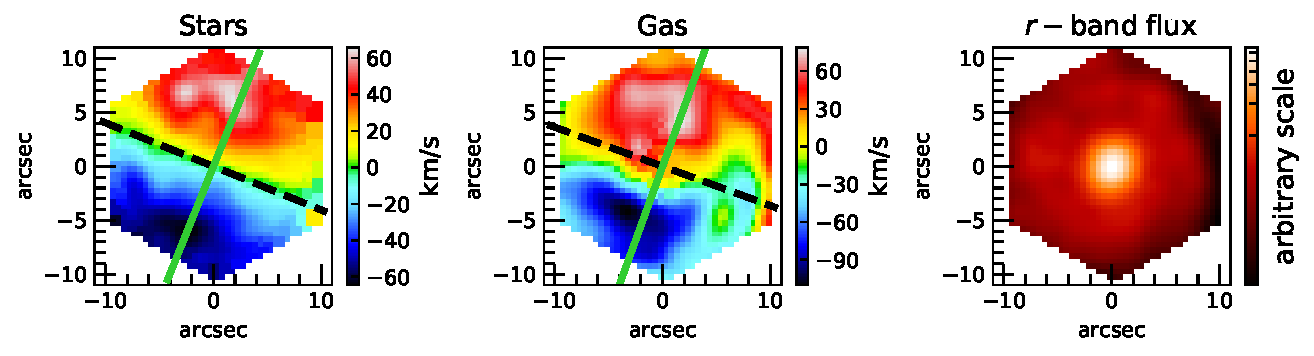
\includegraphics[width=\linewidth]{misalignment_TNG/example_kinematics.pdf}
    \caption{Example outputs from a MaNGA-like observation in TNG100. Shown (left to right) are the stellar velocity field, gas velocity field and normalised $r-$band flux for a given galaxy, `observed' under the same conditions of its MaNGA counterpart (i.e. distance and IFU size). For the stellar and gas velocity fields, the kinematic PA fits (see \S\ref{sec:def_kin_mis}) are shown (green solid line) with the axis of rotation (black dotted line).}
    \label{fig:example_obs}
\end{figure*}

\section{Comparisons to observations} \label{sec:manga_tng_comp}
\subsection{$\Delta$PA}
Firstly we consider all $\Delta$PA defined galaxies for both MaNGA and TNG100. Figure \ref{fig:total_pa_dist} shows the distribution of $\Delta$PA for both MaNGA and IllustrisTNG100. Both distributions are strongly peaked around around 0$^{\circ}$ indicative of the preferentially aligned state predicted from tidal torquing theory. The MaNGA distribution shows a sharp drop-off past 40$^{\circ}$ whereas TNG100 shows a smoother drop off to higher misalignments. Additionally the MaNGA distribution shows a second peak around 180$^{\circ}$ indicative of the stable counter-rotating state identified in previous work \citep[e.g.][]{chen2016}. This secondary peak is not seen for the overall TNG100 sample, however is apparent for star forming galaxies in TNG100 (see bottom panel of Figure \ref{fig:group_morph_PA}). 

\begin{figure}
    \centering
	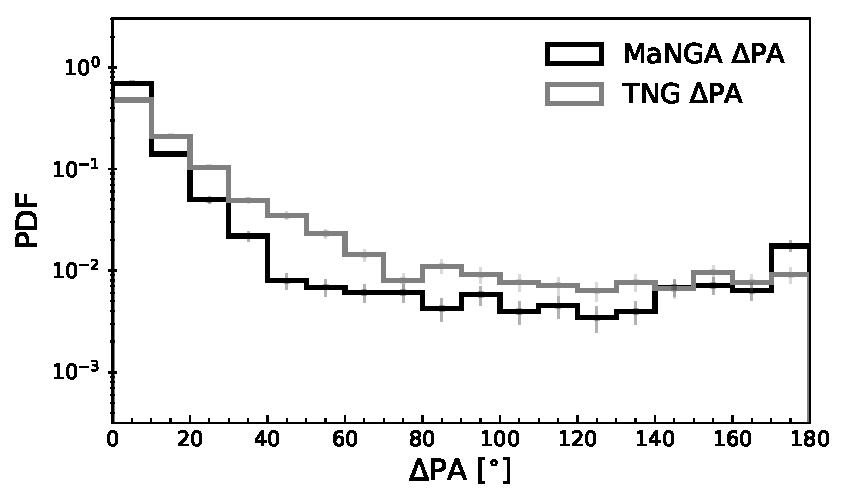
\includegraphics[width=0.85\linewidth]{misalignment_TNG/mpl8_pa_dist.pdf}
    \caption{Probability density distribution of kinematic misalignment as defined by $\Delta$PA for the total MaNGA sample (black line) and matched TNG100 sample (grey line). $\Delta$PA is strongly peaked around 0$^{\circ}$ with a small boost close to 180$^{\circ}$.}
    \label{fig:total_pa_dist}
\end{figure}

The TNG100 mock sample reproduces the general trends well, when considering the differences in how we split the samples in observations and simulations. The smoother drop-off past 40$^{\circ}$ for TNG100 is likely a combination of how we construct the mock observations and scatter in the mass distributions between the MaNGA and TNG100 samples. By construction the matching between MaNGA and TNG100 objects is done before $\Delta$PA is calculated. For this reason there may be differences between the mass distribution of the $\Delta$PA defined MaNGA and TNG100 samples, as shown in Figure \ref{fig:TNG_mpl8_stelM}. We find that the misaligned sample in TNG100 is slightly more massive with respect to MaNGA whereas the aligned samples are consistent. Due to the strong morphological dependence on kinematic misalignment, there is a secondary dependence on stellar mass. The increased overall fraction of misaligned galaxies in TNG100 is therefore, in part, due to the TNG100 $\Delta$PA defined sample being slightly more massive. This slight boost could indicate that the mechanisms for misalignment may be different in simulations than observations. \citet{khim2019} compare the misalignment fractions in observations (SAMI) with simulations (Horizon-AGN). While overall a good agreement is found, they note a significant difference in cluster environments where simulated galaxies are far more likely to be misaligned than in observations. More work needs to be done to understand how well cosmological hydrodynamical simulations replicate the processes leading to misalignment in observations, however, overall trends appear to be well reproduced for different simulation prescriptions.

\begin{figure}
    \centering
	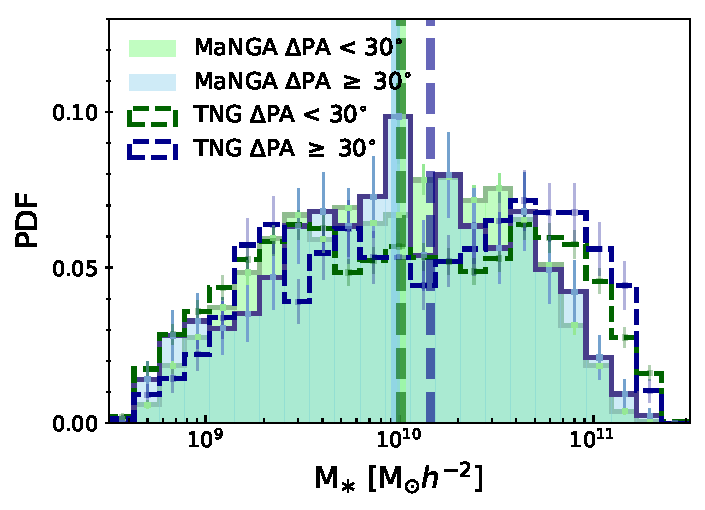
\includegraphics[width=0.85\linewidth]{misalignment_TNG/delPA_split_stelM_tng_comparison.pdf}
    \caption{Probability density distributions of stellar mass, $\mathrm{(M_{\ast}/M_{\odot})}$ for aligned galaxies ($\Delta$PA < 30$^{\circ}$, green) and misaligned galaxies ($\Delta$PA > 30$^{\circ}$, red) defined in MPL-8 (solid lines) and TNG100 (dashed). The vertical lines denote the corresponding distribution's median. The overall distributions are a reasonable match between mocks and observations, with a noted preference for $\Delta$PA defined galaxies at the very high mass end for TNG100. }
    \label{fig:TNG_mpl8_stelM}
\end{figure}

\subsection{Morphological dependence}
We divide our mock MaNGA sample based on the instantaneous star formation rate (SFR) of the galaxy. Here, we define SFR for all gas cells within twice the stellar half mass radius of a given galaxy. The star forming main sequence for all galaxies is found by fitting a power law as a function of stellar mass. A galaxy is then flagged into one of three categories; star forming, green valley or quenched depending on its deviation above or below the main sequence \citep{pillepich2019}. The selected deviations from the main sequence are as follows; star forming galaxy: $\mathrm{\Delta \log_{10}(SFR) > −0.5}$, green valley galaxy: $\mathrm{-1.0 < \Delta \log_{10}(SFR) < -0.5}$ and quenched galaxy: $\mathrm{\Delta \log_{10}(SFR) <= -1.0}$. \red{check this.}

The bottom panel of Figure \ref{fig:group_morph_PA}, shows the $\Delta$PA distribution for the TNG100 sample split into centrals and satellites. Comparing to the observational sample in the top panel of Figure \ref{fig:group_morph_PA}, the morphological trends remain qualitatively the same with quenched/ETGs (star forming/LTGs) more likely to be misaligned (aligned).

Our choice to compare populations split on visual morphology in observations to SFR in simulations is one of necessity. The aim of this work is to explore the relationship of visual morphology with decoupled rotation. Unfortunately we don't currently have the equivalent classifications in IllustrisTNG100, so use an appropriate proxy. In future work, we will look at the relationship between observations and simulations using machine learning classifications of morphology, however, in the following subsections we follow the evolutionary history of the mock sample split by sSFR.

\section{Evolution of angular momentum}
\subsection{Magnitudes}
\red{add more introduction / why you are talking about angular momentum now.}
In this section, we consider the angular momentum content of our TNG100 mock sample back to $z=1$ for stars, gas and dark matter individually. Angular momentum for our TNG100 galaxies is defined by the intrinsic specific angular momentum of their particles/cells:
\begin{equation}
\mathrm{j_{k} = \frac{1}{\sum_{n} m^{(n)}} \sum_{n} m^{(n)}\boldsymbol{x}^{(n)} \times \boldsymbol{v}^{(n)}}
\end{equation}
where $\boldsymbol{v}^{(n)}$ is the velocity of each particle relative to the centre of mass for the galaxy. $\boldsymbol{x}^{(n)}$ is the position of a given particle with respect to the position of the most gravitationally bound particle in the galaxy. We choose this definition since the centre of mass velocity can be biased by structure at large radii in the subhalo/galaxy and hence may spuriously not represent the true rotational centre. $k$ is the particle/cell type referring to either stars, gas or dark matter. For stars and gas this is calculated within a 3D radius equal to the 2D radius corresponding to the angular size of the mock observation. Dark matter is calculated for all particles assigned to the subhalo by the subfind algorithm. 

Figure \ref{fig:sJ_evo} shows the specific angular momentum evolution from $z=1$ for each of stars, gas and DM split on group membership and morphology. We see that similar to the observational sample (see \S\ref{sec:manga_total_pop}), misaligned galaxies in simulations are significantly lower stellar angular momentum than their aligned counterparts at $z=0$. This is reflected in for each of stars, gas and DM to various degrees for all morphologies and central/satellite definition. Interestingly, while misalignment between stars and gas may itself be a transient property, those misaligned at $z = 0$ reside in dark matter haloes with \textit{fundamentally lower angular momentum} which persists to at least $z = 1$. 

\begin{figure*}
	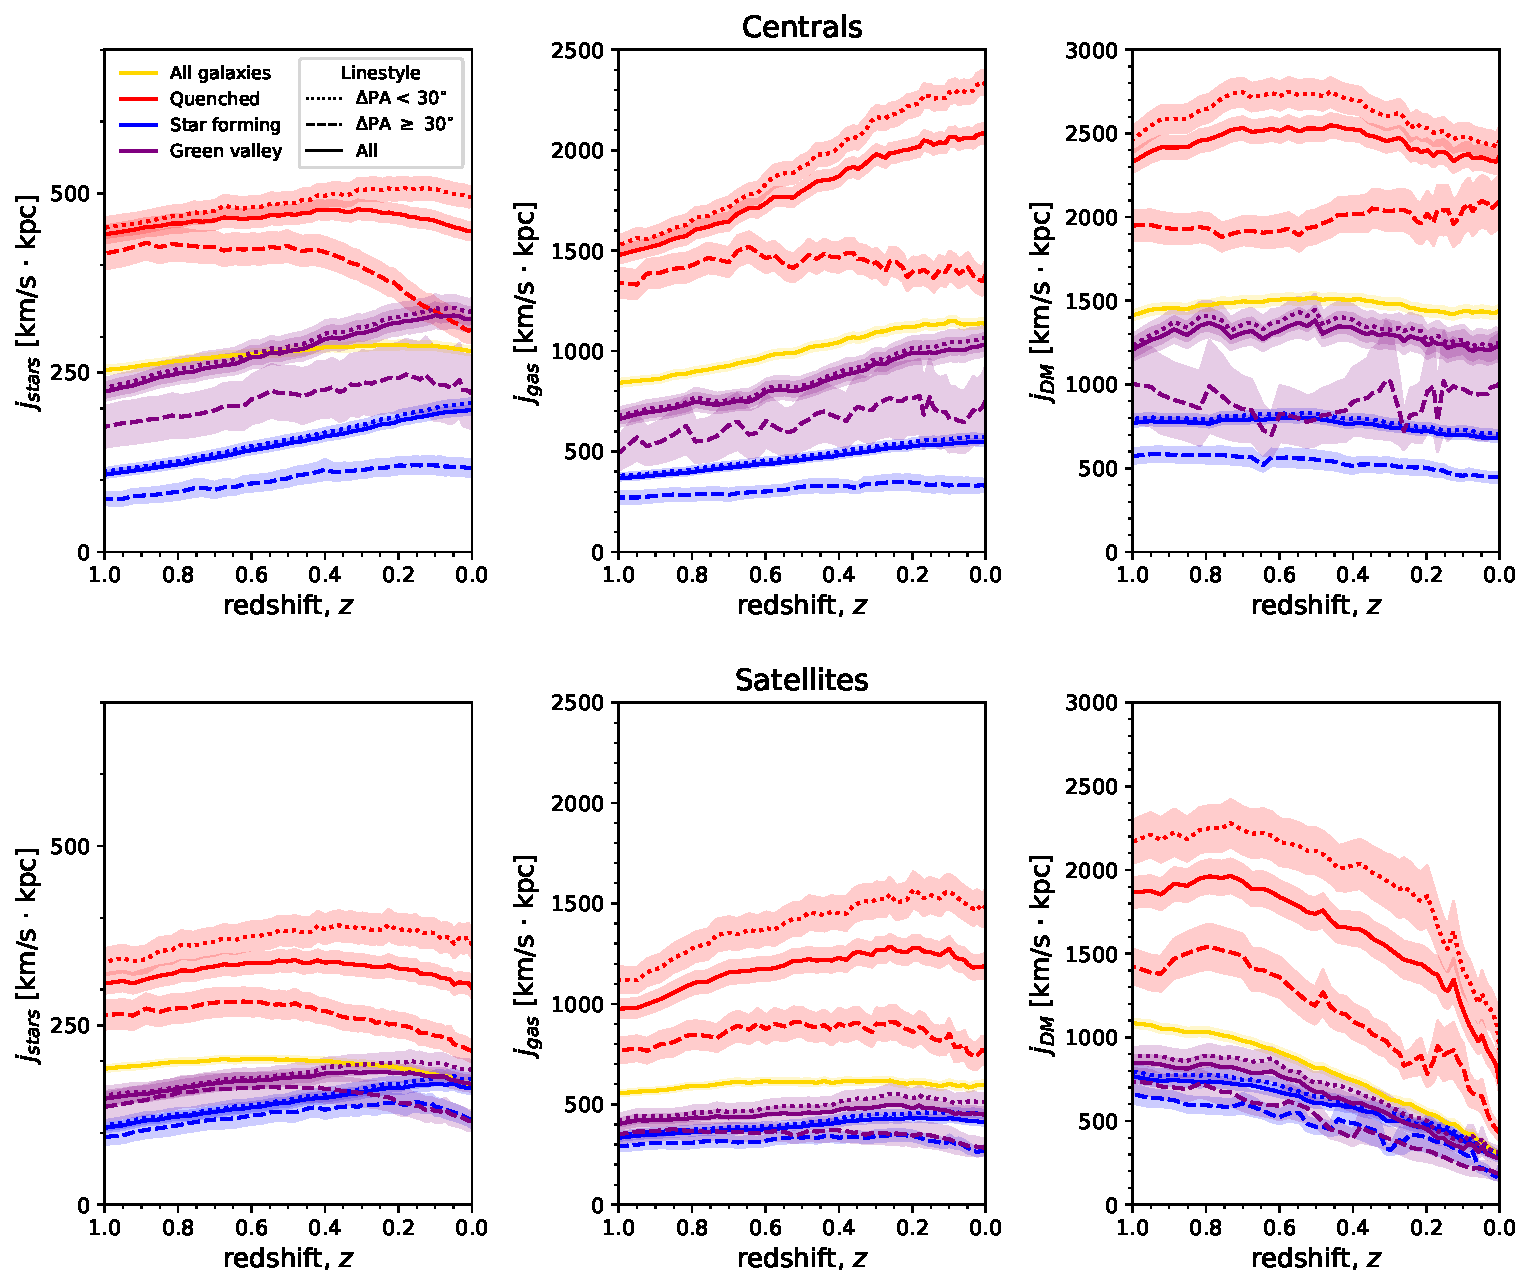
\includegraphics[width=\linewidth]{misalignment_TNG/sJ_evo_cen_sat.pdf}
    \caption{Specific angular momentum evolution from $z = 1$ calculated from star, gas and DM particles (left to right). The angular momentum is calculated for all star and gas particles/cells within the 3D radius assigned by the mock IFU observation, whereas DM is found from all particles associated to the subhalo. The evolution is taken as the median at each timestep for all galaxies of that category with errorbars showing the standard error. The top (bottom) row shows the evolution for central (satellite) galaxies. Each panel displays the evolution split into morphologies; quenched (red), green valley (purple) and star forming (blue) and also $\Delta$PA $< 30^{\circ}$ (dotted) and $> 30^{\circ}$ (dashed). Kinematically misaligned galaxies selected at $z=0$ have notably lower specific angular momentum for all of stars, gas and dark matter.}
    \label{fig:sJ_evo}
\end{figure*}

We note that particle based calculations of specific angular momentum scales with the number of particles. This results in more massive galaxies having higher $\mathrm{j_{i}}$ and further, quenched galaxies (that are typically more massive) having higher $\mathrm{j_{i}}$ than their later type counterparts. While there is only a small difference in-between the mass distributions of our aligned and misaligned samples, to ensure our signal is not simply driven by mass we calculate the residuals of $\mathrm{j_{star}}$ with respect to a typical galaxy of that mass. The residuals, $\Delta \mathrm{j_{star}}$ are calculated by fitting a polynomial to the distribution of $\mathrm{j_{star}}$ vs $\mathrm{M_{\ast}}$ for the galaxies (all mock observations, regardless if $\Delta$PA is well defined) at each snapshot. $\Delta \mathrm{j_{star}}$, is then defined as the deviation of a given galaxy away from the expectation of the fitted line at that mass. Since the trends are qualitatively consistent regardless of morphology, Figure \ref{fig:sJ_evo_residual} shows the specific angular momentum residuals for the total population. For completeness we also include comparison to every galaxy in the mock sample (regardless if $\Delta$PA is well defined). Misaligned galaxies ($\Delta$PA $\geq 30^{\circ}$) for both centrals and satellites show intrinsically lower $\Delta \mathrm{j_{star}}$ with respect to the total population at a given mass, indicative that it is not an effect due to mass. In addition, there is a relative evolution where $\Delta \mathrm{j_{stars}}$ diverges from all galaxies at $z \sim 0.5$ so that misaligned galaxies have even lower stellar angular momentum with respect to the aligned galaxies in recent times.

\begin{figure*}
	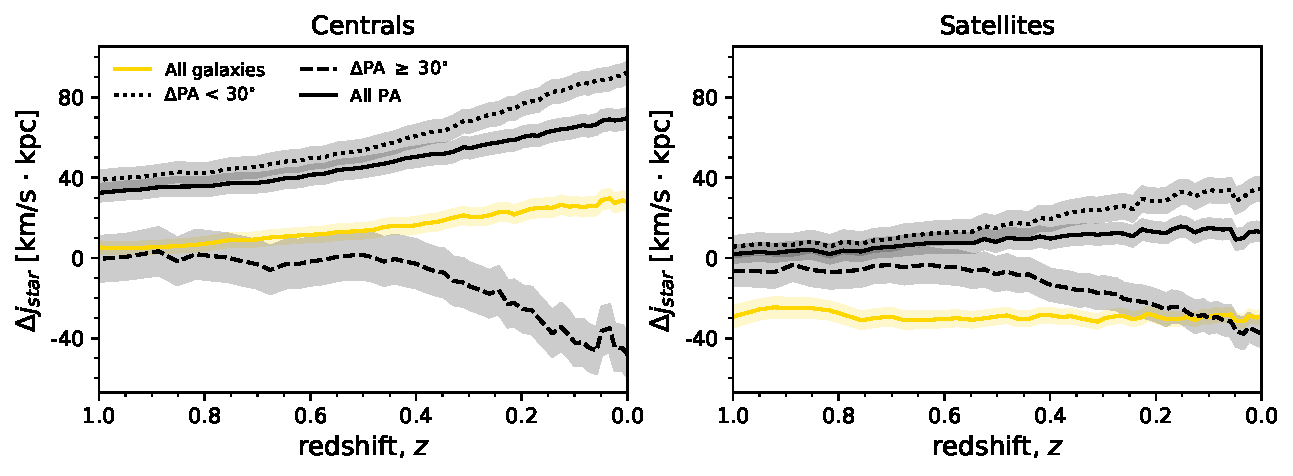
\includegraphics[width=\linewidth]{misalignment_TNG/delta_j_stars_residuals.pdf}
    \caption{The specific angular momentum residuals from $z=1$ for all star particles within the 3D radius assigned by the mock IFU observation. The residual is calculated as the deviation away from the expectation for a galaxy of that mass at each snapshot. The evolution of the residual is taken as the median at each timestep for all galaxies of that category with errorbars showing the standard error. The right (left) panel shows the evolution for central (satellite) galaxies. Each panel displays the evolution for all galaxies (yellow), of which have a defined $\Delta$PA (black solid), aligned galaxies $\Delta$PA $< 30^{\circ}$ (black dotted) and misaligned $> 30^{\circ}$ (black dashed). We see that the difference in angular momentum between aligned and misaligned galaxies is not due to differences in mass. In addition we note a marked deviation of misaligned galaxies to even lower angular momentum in recent times.}
    \label{fig:sJ_evo_residual}
\end{figure*}

\subsection{Direction}
\subsubsection{Computation of 3D angles and comparison to $\Delta$PA}
To conclude this section we now consider the directional 3D offsets between the angular momentum vectors of the stars, gas and dark matter. These are calculated from:
\begin{equation} \label{eq:alpha}
\mathrm{\alpha_{3D} = \text{arccos} \left( \frac{\boldsymbol{j_{i}} \cdot \boldsymbol{j_{j}}}{\left| \boldsymbol{j_{i}} \right| \left| \boldsymbol{j_{j}} \right|} \right),}
\end{equation}
where $i, j$ refer to either stars, gas or dark matter. As for the magnitudes of angular momentum, the star and gas vectors are calculated within a 3D radius set to that of the IFU footprint and the dark matter vector is calculated for all particles assigned to the subhalo by subfind.

A key assumption of this work is the ability for the projected $\Delta$PA to be a reliable estimator of the actual 3D offset between star and gas rotation axes. Figure \ref{fig:PA_residual} shows the distributions of the difference between $\Delta$PA and the 2D and 3D offsets between the angular momentum principal axes of stars and gas. See equation \ref{eq:alpha} for calculation of the 3D offset; the 2D equivalent is simply a projection of this onto the XY plane. $\Delta$PA is a reasonable measure of the true 3D offset which can be modelled as a Gaussian centred on 0$^{\circ}$ with a standard deviation of 17.6$^{\circ}$ (green dotted line). The deviation of the 2D projection from the true 3D offset (black line) has a standard deviation of 13$^{\circ}$, demonstrating that the variation is both due to projection and the noise associated with observations. Additionally, we note the different particle selection for the two measures which may drive slight differences. While the 2D/3D offsets and $\Delta$PA are measured in a footprint with the same radius, the offsets are only defined for particles within a 3D sphere of this radius, where $\Delta$PA is defined for all particles along the line of sight enclosed by the sky footprint. 

\begin{figure}
    \centering
	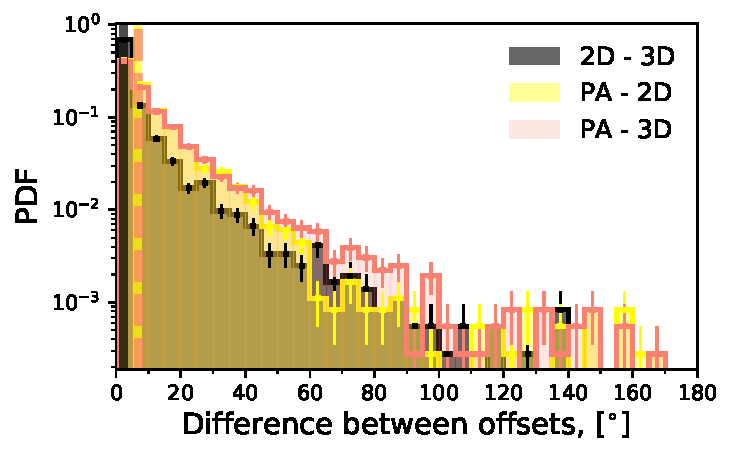
\includegraphics[width=0.9\linewidth]{misalignment_TNG/PA_alpha_resid_hist.pdf}
    \caption{Probability density distribution of the difference between various measures of the star-gas rotational angle offset. The difference between the 3D angular momentum vectors and projection in 2D is shown (black), $\Delta$PA and 2D (yellow) and $\Delta$PA and 3D (red).}
    \label{fig:PA_residual}
\end{figure}

\subsubsection{Results}
Figure \ref{fig:3D_alpha_evo} shows the evolution of the 3D offsets between each of stars, gas and DM respectively. As expected splitting our sample on $\Delta$PA results in significantly higher $\mathrm{\alpha_{STARS - GAS}}$ at $z = 0$ for the misaligned galaxies found in the MaNGA observations. This is also typically correlated, albeit less strongly, with larger $\mathrm{\alpha_{STARS - DM}}$ and $\mathrm{\alpha_{GAS - DM}}$ at $z=0$. This is indicative that a decoupling between stars and gas is often mirrored by a decoupling between the rotation of stars and DM. We also plot the average decoupling for all galaxies (all that are matched to MaNGA) between all components. In the middle panel, we see that $\mathrm{\alpha_{STARS - DM} \sim 50^{\circ}}$ on average for all galaxies (gold line) with a slight redshift evolution which is roughly consistent with previous work \citep[e.g.][]{chisari+17}. We note that our choice to consider the direction of the star and gas rotation within the observational footprint is typically far smaller than the overall DM halo, and hence, may lead to slightly higher typical misalignments between baryonic and DM components.

Working back from $z=0$, we note that $\mathrm{\alpha_{STARS - GAS}}$ for the aligned and misaligned samples (selected at $z=0$) converges in the majority of cases before $z=1$. This indicates the transient nature of misalignment. This is in stark contrast to the magnitude of angular momentum for individual components (stars, gas, DM) which show a persistent difference in magnitude between aligned and misaligned objects (selected at $z=0$) going back past at least $z=1$. 

\begin{figure*}
	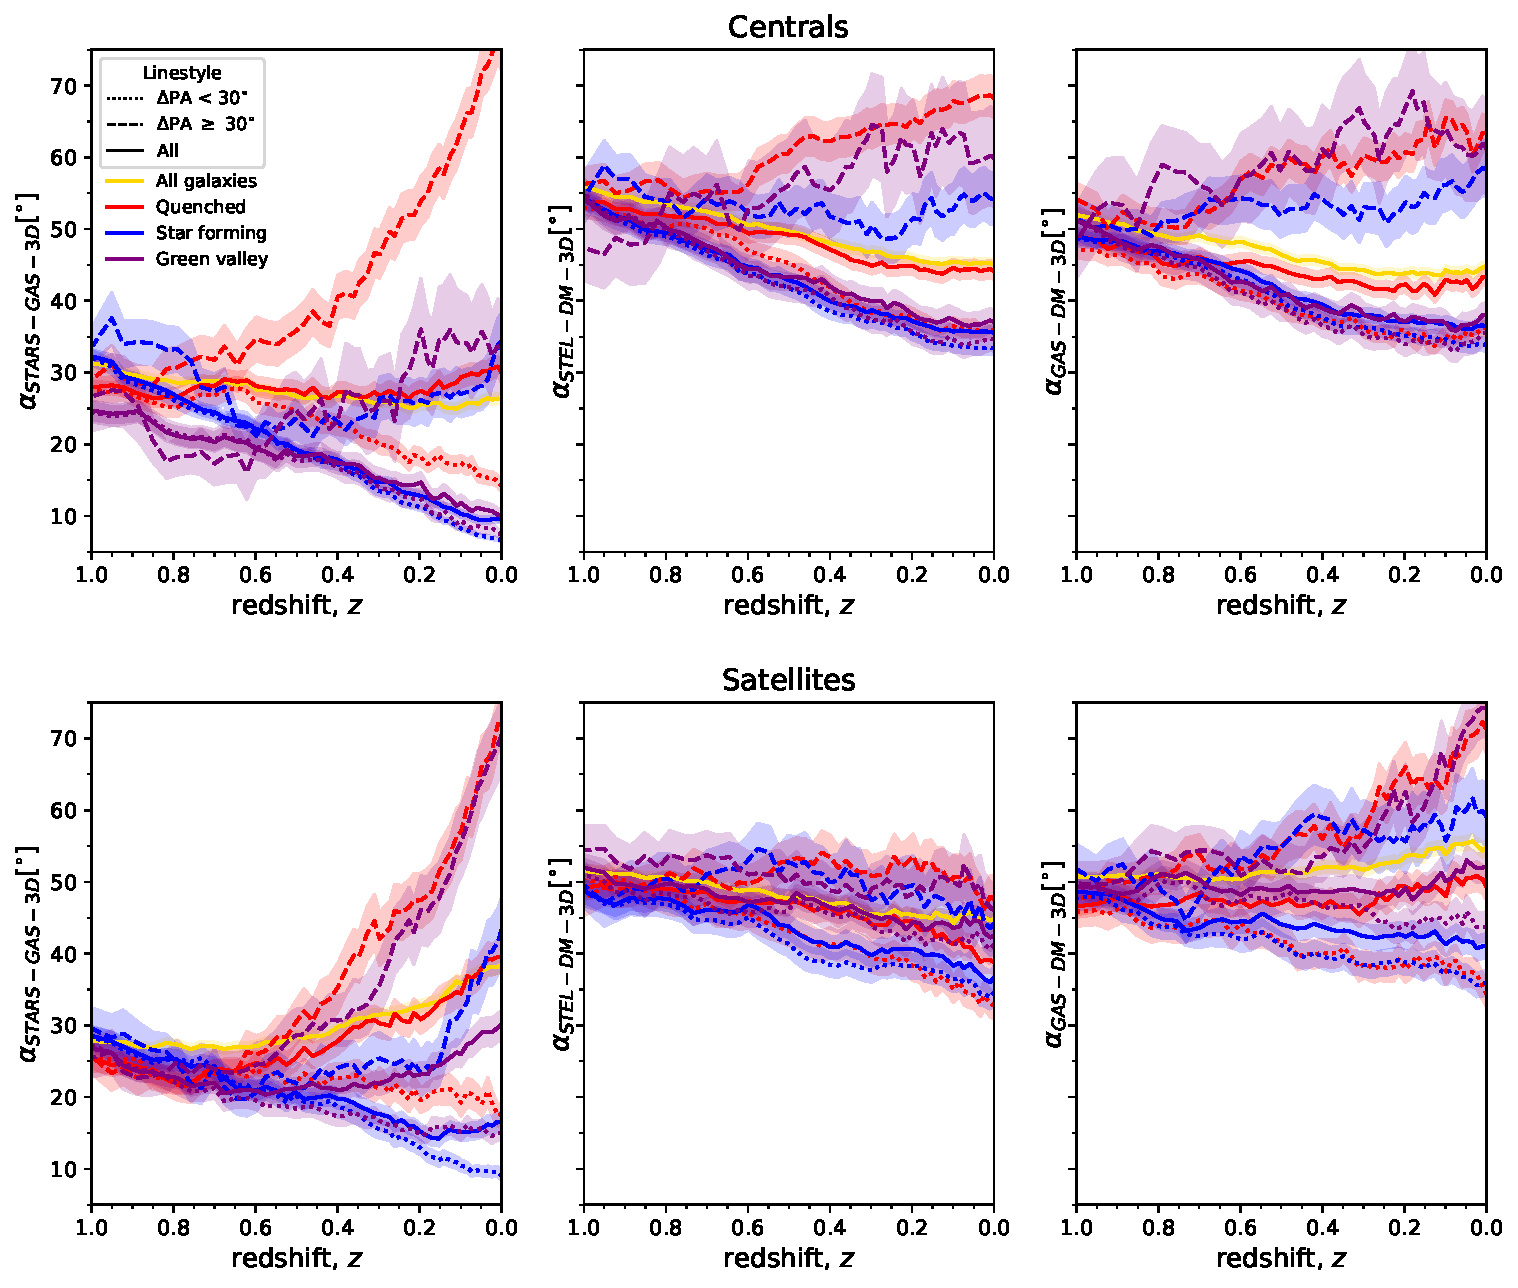
\includegraphics[width=\linewidth]{misalignment_TNG/3D_pa_evo_cen_sat.pdf}
    \caption{Evolution of the 3D offset (in degrees) between the principal spin axes of; stars and gas (left), stars and dark matter (middle) and gas and dark matter (right) from $z=1$. The evolution is taken as the median at each timestep for all galaxies of that category with errorbars showing the standard error. The top (bottom) row shows the evolution for central (satellite) galaxies. Each panel displays the evolution split into morphologies; quenched (red), green valley (purple) and star forming (blue) and also $\Delta$PA $< 30^{\circ}$ (dotted) and $\geq 30^{\circ}$ (dashed).}
    \label{fig:3D_alpha_evo}
\end{figure*}

\section{Discussion}
\red{work out if you want to include the discussion from DI here or if you want an overall discussion for multiple chapters.}

\section{Summary}
In this work, we construct a mock MaNGA sample in IllustrisTNG100 to compare directly to observations and understand the build up of angular momentum in kinematically misaligned galaxies. Our conclusions are as follows:

\begin{enumerate}
    \item We find that a mock MaNGA like sample constructed from cosmological scale hydrodynamical simulation IllustrisTNG100 reproduces the observed trends of decoupling with morphology and stellar angular momentum at $z=0$.
    
    \item We find that decoupled galaxies reside in dark matter haloes with lower spin going back past $z=1$. Despite the decoupling between gas and stars being inherently transient in nature, it is also associated with a decoupling of both stars and gas with respect to dark matter. This demonstrates the inherent link of decoupling, not only to present day stellar angular momentum, but to lower spin haloes at $z=1$. 

\end{enumerate}
In the next chapter, we use our simulated sample to investigate the temporal connection between black hole activity and misalignment in IllustrisTNG100. 